\documentclass{scrartcl}

\usepackage[german]{babel}
\usepackage[utf8]{inputenc}
\usepackage[T1]{fontenc}
\usepackage{listings}
\usepackage{geometry}
\usepackage{graphicx}
\usepackage{fancyhdr}
\usepackage{amsmath}
\usepackage{amssymb}
\usepackage{hyperref}
\usepackage[ruled]{algorithm2e}

\setlength{\parindent}{0pt}
\geometry{left=2.0cm,right=2.0cm,top=2.5cm,bottom=2.5cm}

%
% Fußzeile einstellen
%
\pagestyle{fancy}
\lfoot{Roland Kluge}
\rfoot{19.Dezember 2011}

%
% Umlaute bekanntmachen
%
\lstset{literate=%
{Ö}{{\"O}}1
{Ä}{{\"A}}1
{Ü}{{\"U}}1
{ß}{{\ss}}2
{ü}{{\"u}}1
{ä}{{\"a}}1
{ö}{{\"o}}1
}

\newcommand{\qed}{\ensuremath{\square}}
\newcommand{\landau}[1]{\ensuremath{\mathcal{O}(#1)}}
\newcommand{\capa}{\text{capa}}
\newcommand{\hop}{\text{hop}}

\title{Praktikum 2}
\date{Effiziente Graphenalgorithmen --- WS 2011/2012}
\author{Roland Kluge, 1780358}

\begin{document}

\maketitle

\section{Testdaten}

Die Tests, welche dieser Auswertung zugrunde liegen, können mit dem Skript
\emph{test.sh} nachvollzogen werden.
Die Daten, auf deren Basis argumentiert wird, befinden sich in der Datei
\emph{test\_results.txt} oder in aufbereiteter Form im 
OpenDocument-Spreadsheet \emph{test\_results.ods}.
Sie wurden mit der aktuellen Version der Implementierung mittels der Befehlssequenz
\texttt{qmake spp\_cpp.pro; make release} erstellt und über
10 Testläufe gemittelt.
Die Varianten werden von nun an stets so benannt, wie es auch in der Ausgabe
zu sehen ist.

Die öffentliche Testdatendatei \emph{FLA.sp} wurde so verändert, dass ein
weiterer Knoten eingefügt wurde, der keine Kanten besitzt:
\begin{verbatim}
  v 1070376 82544500 30998800
\end{verbatim}
Dadurch ändert sich natürlich die Kopfzeile:
\begin{verbatim}
  g n 1070377 m 2712798
\end{verbatim}


\section{Übersicht}

Um dies nicht in jedem weiteren Abschnitt zu erwähnen, sei hier angemerkt,
dass es in bestimmten Grenzen natürlich stets auf die Implementierung ankommt, 
ob eine bestimmte Variante schneller ist als eine andere.
Bei den weiteren Aussagen wird dies ignoriert und davon ausgegangen, dass die
vorliegende Implementierung optimal ist.

Die Ergebnisse der 13 relevanten Testfälle ist in Tabelle~\ref{ref:results}
zu sehen. Testfall 13 wurde ausgelassen, da es sich hierbei nur um einen
Grenzfall für einen unverbundenen Graphen mit 2 Knoten handelt.

\begin{figure}[htbp]
%\begin{center}
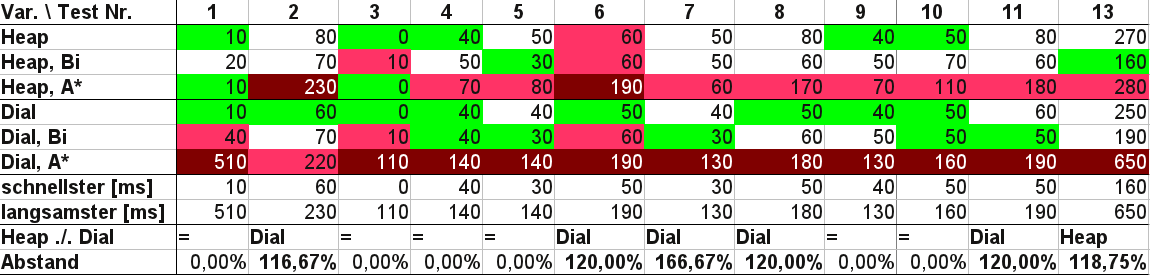
\includegraphics[width=\textwidth]{test_results.png}
%\end{center}
\caption{Übersicht über die Ergebnisse. Grün - beste Laufzeit, Dunkelrot - schlechteste Laufzeit, Pink - zweitschlechteste Laufzeit}
\label{ref:results}
\end{figure}



\section{Dial's Implementierung}

Die Implementierung mit einer einfachen Bucket Queue hat sich als recht 
effizient erwiesen.
In 8 von 13 Tests (entspricht 62\%) war \emph{Dial} am schnellsten, in 
10 von 13 Fällen (entspricht 77\%) war diese Variante unter den besten
beiden Laufzeiten.

\section{Vergleich zwischen Binärem Heap und Bucket Queue}

Setzt man die Implementierungen mit binärem Heap mit der entsprechenden 
Implementierung mittels Bucket Queue  in Beziehung, so erhält man folgendes
Ergebnis, wenn man jeweils das beste Ergebnis der Gruppe betrachtet:

In 6 von 13 Fällen (entspricht 46\%) war die Bucket Queue dem Heap eindeutig überlegen,
in 6 von 13 Fällen (entspricht 46\%) waren beide Gruppen gleich stark und
in 1 von 13 Fällen (entspricht 8\%) war der Heap eindeutig überlegen
 (Zeile \glqq Heap./.Dial\grqq\ in der Tabelle).

Im ersten Fall (BQ vor Heap) war die beste Heap-Implementierung
jeweils 16{,}7\%, 20{,}0\%, 66{,}7\%, 20{,}0\% und 10{,}0\% langsamer als die beste
Bucket Queue-Implementierung, im umgekehrten Fall erhält 
man eine Laufzeitdifferenz von 18{,}8\% (Zeile \glqq Abstand\grqq\ in der Tabelle).

\section{Zielgerichtete Suche}

Beim ersten Betrachten der Ergebnisse fällt auf, dass \emph{Dial, A*} in
11 von 13 Testläufen (85\%) die größe Laufzeit aufweist.
Betrachtet man die zielgerichtete Suche (\emph{$\cdot$,A*}) im Allgemeinen,
dann ist eine der beiden Implementierungen in allen Testläufen am langsamsten.

Bei der Umsetzung von \emph{Dial, A*} trat unter anderem das Problem auf,
dass zunächst einmal die Anzahl der Buckets bestimmt werden musste, wozu
konservativ die Distanzen von allen Knoten zum Ziel berechnet wurden.
Dies erzeugt gerade bei trivialen Grenzfällen einen enormen Overhead
(siehe \emph{Test 1}, hier liegt das Verhältnis von bester zu 
schlechtester Laufzeit bei 1:51), der in $\Theta(n)$ liegt. 

Verglichen mit den anderen 4 Varianten ist ein weiteres Problem, dass die 
Distanzberechnung auf einer Kugel eine verhältnisämßig aufwändige Operation 
ist.

\section{Zufälliges Testen}

Zusätzlich zur Testsuite \emph{test.sh} wurde noch eine Reihe zufälliger
Tests auf dem Graphen \emph{COL.sp} durchgeführt.
Der Befehl dafür lautete:
\begin{verbatim}
  ./Dijkstra ../../prog02/COL.sp -s 0 -t 50 -r
\end{verbatim}
Die Ergebnisse dieses Testlaufs finden sich in der Datei \emph{random\_test.txt},
wobei die Ergebnisse am Ende der Datei Mittelwerte über die Laufzeit und
die Anzahl der PQ-Operationen enthalten.

Man sieht, dass im Mittel \emph{heap, bidirectional} mit rund 62ms am 
schnellsten und \emph{dial, A*} und \emph{heap, A*} mit 291ms bzw.\,148ms am
langsamsten waren.

\section{Fazit}

Nach dieser kurzen Betrachtung können diese Schlussfolgerungen gezogen werden:
\begin{enumerate}
  \item Für die gegebenen Testfälle haben sich die 
        \glqq nicht-beschleunigten\grqq\ Varianten 
        (\emph{Heap},\emph{Dial}) interessanterweise als die überlegenen
        gezeigt.
  \item Tendenziell scheint \emph{Dial} in seinen Varianten \emph{Heap}
        überlegen zu sein, wobei in 50\% der Testfälle eine Übereinstimmung der
        Laufzeiten festgestellt wurde.
  \item Trotz des vielversprechenden heuristischen Ansatzes der zielgerichteten
        Suche, erwies sie sich in diesem Test als die zumeist langsamste 
        Variante, was zum einen auf die komplizierte mathematische Berechnung
        der Potentiale und zum anderen - im Falle von \emph{Dial, A*} - 
        auf die große Zahl leerer Buckets zurückzuführen ist.
\end{enumerate}

Gerade die große Anzahl leerer Buckets könnte reduziert werden, indem man
bspw.\,Radix-Heaps einsetzt oder in einem Bucket nicht nur eine Distanz,
sondern bspw.\,10 Distanzen zulässt, wodurch natürlich eine Priorisierung 
innerhalb des Buckets nötig würde.

\end{document}
